\documentclass[dvipdfmx,aspectratio=169]{beamer}
\usepackage{amsmath}
\usepackage{booktabs}
\usepackage{pxjahyper}
\usepackage{tikz}
\usetikzlibrary{arrows.meta,positioning}

\usetheme{Madrid}
\usecolortheme{default}
\setbeamertemplate{navigation symbols}{}

\title{AtCoder Beginner Contest 454 -- C\\\small Straw Millionaire の解説}
\author{}
\date{}

\begin{document}

\begin{frame}
  \titlepage
\end{frame}

\begin{frame}{問題の概要}
  \begin{itemize}
    \item アイテム $1, 2, \ldots, N$ の $N$ 種類がある．
    \item 高橋君は最初\textbf{アイテム 1} のみを所持．
    \item $M$ 人の友達がいて，$i$ 番目の友達は
      「\textbf{アイテム $A_i$ を渡すとアイテム $B_i$ をもらえる}」
      という交換をしてくれる．
    \item 高橋君が\textbf{手に入れることのできるアイテム}は何種類あるか？
      （アイテム 1 を含める）
  \end{itemize}

  \vspace{0.8em}
  \textbf{制約}: $2 \le N \le 3 \times 10^5$,\quad $1 \le M \le 3 \times 10^5$,\quad $A_i \ne B_i$
\end{frame}

\begin{frame}{サンプル 1 を手で動かす}
  \[
    N=5,\; M=5,\quad
    (A_i, B_i) = (1,2),\,(2,3),\,(3,4),\,(2,4),\,(5,2)
  \]

  \vspace{0.6em}
  交換の可能性を追う：
  \begin{itemize}
    \item アイテム 1 を持っている $\Rightarrow$ 友達 1 で\textbf{アイテム 2} を入手可
    \item アイテム 2 を持てば $\Rightarrow$ 友達 2 で\textbf{アイテム 3}，友達 4 で\textbf{アイテム 4}
    \item アイテム 3 を持てば $\Rightarrow$ 友達 3 で\textbf{アイテム 4}（既にあり）
    \item アイテム 5 からしか出ない交換（友達 5）は使えない（5 を持てない）
  \end{itemize}

  \vspace{0.6em}
  \begin{alertblock}{答え}
    到達できたアイテム: $\{1, 2, 3, 4\}$ → \textbf{4 種類}
  \end{alertblock}
\end{frame}

\begin{frame}{なぜ「グラフ」を思いつくか --- 問題文の読み方}
  問題文の\textbf{構造だけ}を書き出してみる：

  \vspace{0.6em}
  \begin{block}{問題の本質}
    \begin{itemize}
      \item \textbf{対象}：アイテム（離散的，$N$ 個）
      \item \textbf{関係}：「$A_i$ を持てば $B_i$ も手に入る」という\textbf{一方向の}条件
      \item \textbf{連鎖}：$B_i$ を得たら，今度は $B_i$ を前提とする別の交換ができる
      \item \textbf{始点}：アイテム 1
      \item \textbf{問い}：始点から\textbf{「届く」もの}は何個？
    \end{itemize}
  \end{block}

  \vspace{0.6em}
  この 5 つが揃ったら，\textbf{有向グラフの到達可能性問題}のサイン．
\end{frame}

\begin{frame}{典型パターンへの翻訳}
  「\textbf{A があれば B が得られる}」型の問題は，次のように翻訳する：

  \vspace{0.8em}
  \begin{center}
    \begin{tabular}{ll}
      \toprule
      問題の言葉 & グラフの言葉 \\
      \midrule
      アイテム $i$ & 頂点 $i$ \\
      「$A_i$ を渡すと $B_i$ がもらえる」 & 有向辺 $A_i \to B_i$ \\
      最初に持っているもの & 始点 $s = 1$ \\
      手に入れられる種類数 & $s$ から到達可能な頂点数 \\
      \bottomrule
    \end{tabular}
  \end{center}

  \vspace{0.8em}
  \begin{block}{思考の合言葉}
    「\textbf{A → B} の矢印が頭に浮かんだらグラフを描く」
  \end{block}
\end{frame}

\begin{frame}{サンプル 1 をグラフで見る}
  \begin{center}
    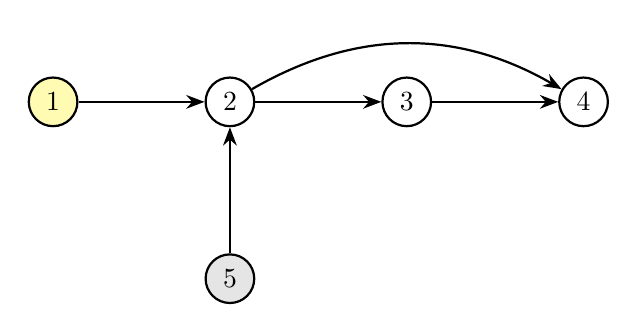
\begin{tikzpicture}[>=Stealth, node distance=1.6cm, thick]
      \node[circle,draw,fill=yellow!30] (1) {1};
      \node[circle,draw,right=of 1] (2) {2};
      \node[circle,draw,right=of 2] (3) {3};
      \node[circle,draw,right=of 3] (4) {4};
      \node[circle,draw,fill=gray!20,below=of 2] (5) {5};

      \draw[->] (1) -- (2);
      \draw[->] (2) -- (3);
      \draw[->] (3) -- (4);
      \draw[->] (2) to[bend left=30] (4);
      \draw[->] (5) -- (2);
    \end{tikzpicture}
  \end{center}

  \vspace{0.4em}
  \begin{itemize}
    \item 黄色 = 始点 1．そこから\textbf{矢印で辿れる}頂点は $\{1,2,3,4\}$．
    \item 頂点 5 は始点からは到達不能．
  \end{itemize}

  \begin{alertblock}{到達可能な頂点数 = 4 = 答え}
  \end{alertblock}
\end{frame}

\begin{frame}{公式解説のアルゴリズム（BFS）}
  $N$ 頂点・$M$ 辺の有向グラフで，頂点 1 から到達可能な頂点数を求める．

  \vspace{0.6em}
  \begin{block}{手順（幅優先探索 BFS）}
    \begin{itemize}
      \item 到達済み集合 $S$ をもつ．初期値 $S = \{1\}$．
      \item 探索待ちのキュー $q$ をもつ．初期値 $q = [1]$．
      \item $q$ が空でない間：
        \begin{itemize}
          \item $q$ から 1 つ取り出して $x$ とする．
          \item $x$ から出る辺の先 $y$ について：
            \begin{itemize}
              \item $y \in S$ ならスキップ．
              \item そうでなければ $S$ と $q$ に $y$ を入れる．
            \end{itemize}
        \end{itemize}
      \item 最後に $|S|$ が答え．
    \end{itemize}
  \end{block}

  実装上は $S$ を長さ $N+1$ の \texttt{bool} 配列，$q$ を \texttt{queue} で持つのが定番．
\end{frame}

\begin{frame}{「渡すと失うのでは？」という疑問への答え}
  素直に読むと「\textbf{$A_i$ を渡す}」は $A_i$ を失うように見える．
  が，本問では到達可能性でよい．その理由：

  \vspace{0.6em}
  \begin{itemize}
    \item 求めるのは「手に入れる\textbf{ことのできる}アイテムの種類数」．
      \textbf{最終所持数ではなく，一度でも入手できれば良い}．
    \item グラフで 1 から $v$ へ経路 $1 \to u_1 \to \cdots \to v$ があれば，
      順次交換することで途中のアイテムを\textbf{全部一度ずつ入手できる}．
    \item 到達可能な頂点集合だけが「一度でも所持しうる」候補．
      それ以外は絶対に入手できない．
  \end{itemize}

  \vspace{0.6em}
  \begin{block}{サンプル 3 の検算（答え 6）}
    辺: $2\to 6,\,2\to 5,\,3\to 6,\,1\to 6,\,1\to 2,\,5\to 6,\,2\to 3,\,3\to 7$\\
    1 から到達可能: $\{1,2,3,5,6,7\}$（頂点 4 は孤立）$\Rightarrow$ \textbf{6}．
  \end{block}
\end{frame}

\begin{frame}[fragile]{実装：C++}
\begin{verbatim}
int n, m;
cin >> n >> m;
vector<vector<int>> g(n + 1);
for (int i = 0; i < m; i++) {
    int a, b; cin >> a >> b;
    g[a].push_back(b);           // A -> B の有向辺
}

vector<bool> seen(n + 1, false);
queue<int> q;
q.push(1); seen[1] = true;
int ans = 0;
while (!q.empty()) {
    int u = q.front(); q.pop();
    ans++;
    for (int v : g[u])
        if (!seen[v]) { seen[v] = true; q.push(v); }
}
cout << ans << endl;
\end{verbatim}
\end{frame}

\begin{frame}[fragile]{実装：PyPy}
\begin{verbatim}
import sys
from collections import deque

def main():
    data = sys.stdin.buffer.read().split()
    it = iter(data)
    n = int(next(it)); m = int(next(it))
    g = [[] for _ in range(n + 1)]
    for _ in range(m):
        a = int(next(it)); b = int(next(it))
        g[a].append(b)

    seen = [False] * (n + 1)
    seen[1] = True
    q = deque([1])
    ans = 0
    while q:
        u = q.popleft(); ans += 1
        for v in g[u]:
            if not seen[v]:
                seen[v] = True
                q.append(v)
    print(ans)

main()
\end{verbatim}
\end{frame}

\begin{frame}{計算量}
  \begin{itemize}
    \item 辺の構築：$O(M)$
    \item BFS：各頂点 1 回，各辺 1 回訪問するので $O(N + M)$
  \end{itemize}

  \vspace{0.8em}
  全体で $\mathbf{O(N + M)}$．\par
  $N, M \le 3 \times 10^5$ なので十分高速．

  \vspace{0.8em}
  \begin{block}{注意点}
    \begin{itemize}
      \item DFS を再帰で書くと $N$ 大で\textbf{スタックオーバーフロー}の恐れ．
        BFS（キュー）か，スタックを陽に持つ反復 DFS が安全．
      \item 多重辺・自己ループの可能性は薄いが，$A_i \ne B_i$ は制約で保証．
    \end{itemize}
  \end{block}
\end{frame}

\begin{frame}{まとめ}
  \begin{enumerate}
    \item 「\textbf{$A$ を持てば $B$ が得られる}」型は有向グラフで定式化．
    \item 始点から「届くもの」を問われたら\textbf{到達可能性} → BFS/DFS．
    \item 計算量 $O(N+M)$ で制約内．
  \end{enumerate}

  \vspace{1em}
  \begin{block}{覚えること}
    問題文を読んで次の 3 点が揃ったら，まずグラフを描く：\\
    \textbf{対象} × \textbf{一方向の関係} × \textbf{連鎖的な到達}．
  \end{block}
\end{frame}

\end{document}
